\section{Fourierreihen}

% 22-10-2019 (Teil 2) - BEGIN 
%%%%%%%%%%%%%%%%%%%%%%%%%%%%%%%%%%%%%%%%%%%%%%%%%%%%%%%%%%%%%%%%%%%%%%%%%%%%%%%%%%%%%%%%%%%%%%%%%%%
Temperaturverteilung auf Ring
$$a_0 + \sum_0^\infty (a_n \cos(n\omega\phi) + b_n \sin(n\omega\phi))$$

P.L. Dirichlet (1829) $\rightarrow$ mathematischer Beweis

Zerlegung einer periodischen Funktion nach diskreten Teilfrequenzen
\begin{itemize}
	\item Fourieranalyse
	\item Fouriersynthese
\end{itemize}

Periodische Funktion mit Periodenlänge $L$
\begin{figure}[H]
	\centering
	\includegraphics[width=0.7\linewidth]{Grafiken/2_Fourierreihen/Grafik1.PNG}
	\caption{Periodische Funktion mit Periodenlänge $L$}
	\label{}
\end{figure}

\begin{Def}
	Eine Funktion $f: \mathbb{R}\rightarrow\mathbb{R}(\mathbb{C})$ wird periodischen
	mit Periode $L$ , $L>0$, genannt wenn:
	$$f(x+L) = f(x) \quad \forall x \in \mathbb{R}$$
\end{Def}

\begin{Bem}
	Periodiesche Funktion mit Periode $L$ ist eindeutig auf ganz $\mathbb{R}$ fesgelegt,
	wenn man sie auf einem beliebiges Intervall der Länge $L$, $[a,a+L)$ kennt.\\
	Standardvorgabe:
	$$[0,L) \quad \textrm{oder} \quad [-\frac{L}{2}, \frac{L}{2})$$
\end{Bem}

\begin{Bem}
	$f(x)$ periodisch mit Periode $L$
	$$\Rightarrow \int_{-\frac{L}{2}}^{\frac{L}{2}} \,dx f(x) = \int_{a-\frac{L}{2}}^{a+\frac{L}{2}} \,dx f(x)$$
\end{Bem}

Betrachte Funktion $f: \mathbb{R}\rightarrow\mathbb{R}(\mathbb{C})$ mit
\begin{enumerate}[label=(\roman*)]
	\item periodisch mit Periode L, d.h. $f(x+L) = f(x) \quad \forall x \in \mathbb{R}$
	\item Lebesque-integrierbar auf dem Periodizitätsintervall, dh $f \in L^1(-\frac{L}{2},\frac{L}{2})$ (schwächer als quadratintegrierbar)
\end{enumerate}

Betrachte Funktionen der Einfachheit halber für $L=2\pi$\\
Die $\infty$-trigometrische Reihe
$$FR(f)(x)= \frac{1}{2} a_0 + \sum_{n=1}^\infty (a_n \cos(n x) + b_n \sin(n x)) \quad \textrm{mit}$$
$$a_n = \frac{1}{\pi} \int_{-\pi}^{\pi} \,dx f(x)\cos(nx) \quad n \geq 0 \quad n \in \mathbb{N}$$
$$b_n = \frac{1}{\pi} \int_{-\pi}^{\pi} \,dx f(x)\sin(nx) \quad n>0 \quad n \in \mathbb{N}$$
heißt Fourierreihe der Funktion $f$ mit den Fourierkoeffizienten $a_n$ und $b_n$.

Konvergenz der Partialsummen

$FR(f)(x)= \frac{1}{2} a_0 + \sum_{n=1}^N (a_n \cos(n x) + b_n \sin(n x))$

muss beachtet werden.

\begin{Bem}
	Wenn $f \in L^1(-\pi,\pi)$, dann stellt Fourierreihe eine Entwicklung nach der
	OGB

	$\{1, \sin(nx), \cos(nx); n \in \mathbb{N}\}$ auf $\sqrt{2}$ normiert $\Rightarrow \frac{1}{2}$ bei $a_0$

	bzgl. des Skalarprodukts

	$$\langle f,g \rangle =  \frac{1}{\pi} \int_{-\pi}^{\pi} \,dx \overline{f(x)} g(x)$$

	dar.

	$\Rightarrow FR(f)$ konvergiert in $L^2$-Norm (Konvergenz im Mittel)

	$$\lim_{n\rightarrow \infty} {\Vert f- FR_N(t) \Vert}_2 = 0$$
\end{Bem}

\begin{Satz}{Parsewal I}
	$$\Vert f \Vert^2 = \frac{1}{2} \vert a_0 \vert^2 + \sum_{n=1}^{\infty} \left(\vert a_n \vert^2 + \vert b_n \vert^2\right)$$
\end{Satz}

%%%%%%%%%%%%%%%%%%%%%%%%%%%%%%%%%%%%%%%%%%%%%%%%%%%%%%%%%%%%%%%%%%%%%%%%%%%%%%%%%%%%%%%%%%%%%%%%%%%
% 22-10-2019 (Teil 2) - END

% 24-10-2019 - BEGIN 
%%%%%%%%%%%%%%%%%%%%%%%%%%%%%%%%%%%%%%%%%%%%%%%%%%%%%%%%%%%%%%%%%%%%%%%%%%%%%%%%%%%%%%%%%%%%%%%%%%%
\subsubsection{Rechenregeln und Beispiele}
\begin{enumerate}[label=(\roman*)]
	\item Allgemeines Periodizitätsintervall $(a,b)$
		$$FR(f)(x)= \frac{1}{2} a_0 + \sum_{n=1}^\infty \left( a_n \cos\left(\frac{2\pi n x}{b-a}\right) + b_n \sin\left(\frac{2\pi n x}{b-a}\right) \right)$$
		$$a_n = \frac{2}{b-a} \int_{a}^{b} \,dx f(x) \cos \left(\frac{2\pi n x}{b-a}\right) \quad n \geq 0$$
		$$b_n = \frac{2}{b-a} \int_{a}^{b} \,dx f(x) \sin \left(\frac{2\pi n x}{b-a}\right) \quad n>0$$	

	\item Integrale über ein symetrisches Integrationsintervall 
		$\left(-\frac{L}{2}, \frac{L}{2} \right)$ um Null verschwinden
		für ungerade Integranden:
		\begin{itemize}
			\item $f(x) \quad \textrm{ungerade} \Leftrightarrow f(x) = -f(-x)$ 
				$$\frac{2}{L} \int_{-\frac{L}{2}}^{\frac{L}{2}} \,dx \underbrace{\underbrace{f(x)}_{ungerade} \underbrace{\cos\left(\frac{2\pi}{L} n x\right)}_{gerade}}_{ungerade} = 0 \quad \cos()\textrm{-Terme verschwinden}$$
			\item $f(x) \quad \textrm{gerade} \Leftrightarrow f(x) = f(-x)$
				$$\frac{2}{L} \int_{-\frac{L}{2}}^{\frac{L}{2}} \,dx \underbrace{\underbrace{f(x)}_{gerade} \underbrace{\sin\left(\frac{2\pi}{L} n x\right)}_{ungerade}}_{ungerade} = 0 \quad \sin()\textrm{-Terme verschwinden}$$
		\end{itemize}
	\item Integrale über ein Vielfaches der Periode von $\sin$- oder 			$\cos$-Funktion verschwinden
		$$\int_{a}^{a+k\frac{L}{n}} \sin\left(\frac{2\pi}{L} n x\right) \,dx =
		\int_{a}^{a+k\frac{L}{n}} \cos\left(\frac{2\pi}{L} n x\right) \,dx = 0
		\quad k\neq 0 \quad n \neq 0$$
		\begin{figure}[H]
			\centering
			\includegraphics[width=0.4 \linewidth]{Grafiken/2_Fourierreihen/Grafik2.PNG}
		\end{figure}
	\item Linearität der Fourierreihe
		$$FR(f+g)(x) = FR(f)(x) + FR(g)(x)$$
		$$FR(\alpha \cdot f)(x) = \alpha \cdot FR(f)(x)$$
\end{enumerate}

\begin{Bsp}{Sägezahnfunktion}
	$$f(x)=x \quad x \in (-\pi,\pi) \quad \textrm{Periode: } 2\pi$$
	\begin{figure}[H]
		\centering
		\includegraphics[width=0.4\linewidth]{Grafiken/2_Fourierreihen/Grafik3.PNG}
	\end{figure}

	$$a_{n \geq 0} = \frac{1}{\pi} \int_{-\pi}^{\pi} \,dx x \cos(nx) = 0$$
	
	$$
	b_{n > 0} = \frac{1}{\pi} \int_{-\pi}^{\pi} \,dx x \sin(nx)
		= \left. - \frac{x}{n \pi} \cos(nx) \right\vert_{-\pi}^\pi
			+ \int_{-\pi}^{\pi} \,dx \cos(nx)
		= - \frac{2 \pi}{n \pi} \cos(n\pi)
		= \frac{2}{n} = (-1)^{n-1}
	$$

	$$FR(f)(x) = 2 \sum_{n=1}^\infty \frac{1}{n} (-1)^{n+1} \sin(nx)$$
	$$\rightarrow FR \textrm{ konvergiert in } L^2\textrm{-Norm gegen } f$$

	Ableitung der Fourierreihe:
	$$\frac{d}{dx} FR(f)(x) = 2 \sum_{n=1}^\infty (-1)^{n+1} \cos(nx) \quad \rightarrow
	\textrm{ divergente Reihe \textbf{!}}$$
\end{Bsp}

\begin{Bsp}{$f(x)=\frac{x}{b} \qquad x \in (0,b) \textrm{ mit Periode } b$}
	
	\begin{tabular}{ll}
		Kennen:	& $FR(g)(y)$ für $g(y)=y \qquad y \in (- \pi , \pi)$ \\
				& $FR(g)(y) = 2 \sum_{n=1}^\infty \frac{(-1)^{n+1}}{n} \sin(y)$
	\end{tabular}

	$y = \frac{2 \pi}{b} x - \pi$

	$$
	\left.
	\begin{array}{l}
		f(0) = 0 \quad g(y(0)) = g(-\pi) = -\pi \\
		f(b) = 1 \quad g(y(b)) = g(\pi) = \pi \\
	\end{array}
	\right\}
	\Rightarrow g = 2\pi f - \pi \quad \Rightarrow \quad f = \frac{1}{2\pi}g + 
	\frac{1}{2}
	$$

	$$
	FR(f)(x) = \frac{1}{2} + \frac{1}{2\pi} FR(g)(y(x))
		= \frac{1}{2} + \frac{1}{2\pi} 2 \sum_{n=1}^\infty \frac{(-1)^{n+1}}{n}
			\sin\left( n \left( \frac{2\pi}{b}x-\pi \right) \right)
		= \frac{1}{2} - \frac{1}{\pi} \sum_{n=1}^\infty \frac{1}{n}
			\sin \left( \frac{2\pi}{b} n x \right)
	$$

\end{Bsp}

\begin{Satz}
	Ist eine periodische Funktion $f$, die auf dem Periodizitätsintervall
	$[-\frac{L}{2}, \frac{L}{2}]$ stückweise stetig diff-bar ($f$ ist auf
	$(-\frac{L}{2}, \frac{L}{2})$ diff-bar und $f'$ ist auf $(-\frac{L}{2}, \frac{L}{2})$
	stückweise stetig), auf ganz ganz $\mathbb{R}$ stetig ist, so gilt im
	Differenzierbarkeitsbereich von f

	$$FR(f')(x) = \underbrace{\frac{d}{dx}FR(f)(x)}_{termweise \quad Ableitung}$$

\end{Satz}

\begin{Bem}
	Konvergiert $\frac{d}{dx} FR(f)(x)$ gleichmäßig $\Rightarrow$
	Grenzfunktion ist stetige Funktion die auf $[-\frac{L}{2}, \frac{L}{2}]$
	mit $f'(x)$ übereinstimmt
\end{Bem}

\begin{Satz}
	$f(x)$ stückweise diff-bare Funktion auf $[-\frac{L}{2}, \frac{L}{2}]$ mit
	Fourierreihe $FR(f)(x)$, wobei $a_0 = 0$ und Stammfunktion $F(x)$.
	Dann gilt:
	$$FR(f)(x) = \underbrace{\int \,dx FR(f)(x)}_{termweise \quad Integration} $$
\end{Satz}

\subsubsection{Konvergenz von Fourierreihen}
\textbf{Konvergenz im Mittel (Konvergenz in $L^2$-Norm)}
$$\lim_{N \rightarrow \infty} \Vert FR_N(f)-f \Vert_2 = 0$$

\textbf{Punktweise Konvergenz}
$$\lim_{N \rightarrow \infty} \vert FR_N(f)(x)-f(x) \vert = 0$$

\textbf{Gleichmäßige Konvergenz}
$$\lim_{N \rightarrow \infty} \Vert FR_N(f)-f \Vert_\infty = \lim_{N \rightarrow \infty} 
\max_{x \in [-\frac{L}{2} , \frac{L}{2}]} \vert FR_N(f)(x)-f(x) \vert = 0$$

mit $FR_N(f)(x) = \frac{1}{2} a_0 + \sum_{n=1}^N(a_n \cos(x) + b_n \sin(x)$

%%%%%%%%%%%%%%%%%%%%%%%%%%%%%%%%%%%%%%%%%%%%%%%%%%%%%%%%%%%%%%%%%%%%%%%%%%%%%%%%%%%%%%%%%%%%%%%%%%%
% 24-10-2019 - END

% 29-10-2019 - BEGIN 
%%%%%%%%%%%%%%%%%%%%%%%%%%%%%%%%%%%%%%%%%%%%%%%%%%%%%%%%%%%%%%%%%%%%%%%%%%%%%%%%%%%%%%%%%%%%%%%%%%%
\begin{Bsp}{Funktionenfolge $f_n(x)=x^n$ \qquad $x \in [0,1]$}
	$$
	\lim_{n \rightarrow \infty} = \left\{ \begin{array}{ll}
        0 & x \in [0,1) \\
        1 & x = 1 \\
        \end{array}
		\right.
	$$

	\textbf{Punktweise Konvergenz}
	$$\forall \epsilon > 0 \quad \forall x \in D \, \exists \, N(\epsilon, x) :
		\vert f_n(x)-f(x) \vert < \epsilon \quad, n > N(\epsilon,x)$$

	$ \underline{x = 1:} \quad N(\epsilon,x) = 1$

	$ \underline{x \in [0,1):}$

\end{Bsp} 


\begin{figure}[H]
	\centering
	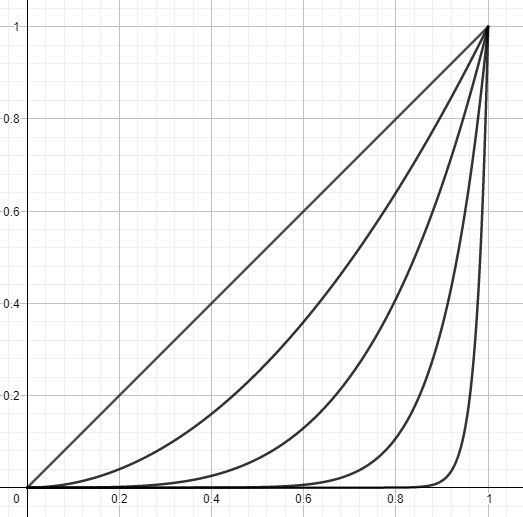
\includegraphics[width=0.4\linewidth]{Grafiken/2_Fourierreihen/Grafik4.PNG}
\end{figure}



\subsubsection{Komplexe Form der Fourierreihe}



%%%%%%%%%%%%%%%%%%%%%%%%%%%%%%%%%%%%%%%%%%%%%%%%%%%%%%%%%%%%%%%%%%%%%%%%%%%%%%%%%%%%%%%%%%%%%%%%%%%
% 29-10-2019 - END

% 31-10-2019 (Teil 1) - BEGIN 
%%%%%%%%%%%%%%%%%%%%%%%%%%%%%%%%%%%%%%%%%%%%%%%%%%%%%%%%%%%%%%%%%%%%%%%%%%%%%%%%%%%%%%%%%%%%%%%%%%%
\subsubsection{Fourier-Cosinus und Fourier-Sinus-Reihe}

%%%%%%%%%%%%%%%%%%%%%%%%%%%%%%%%%%%%%%%%%%%%%%%%%%%%%%%%%%%%%%%%%%%%%%%%%%%%%%%%%%%%%%%%%%%%%%%%%%%
% 31-10-2019 (Teil 1) - END